\section{Installing and connecting Griffin to PostgreSQL}
\subsubsection{Tool installation}
To install Apache Griffin and make the configurations, we used the following architecture:
\begin{figure}[H]
    \caption{Architecture implemented to test Apache Griffin}  \label{fig:xray}
    \begin{center}
      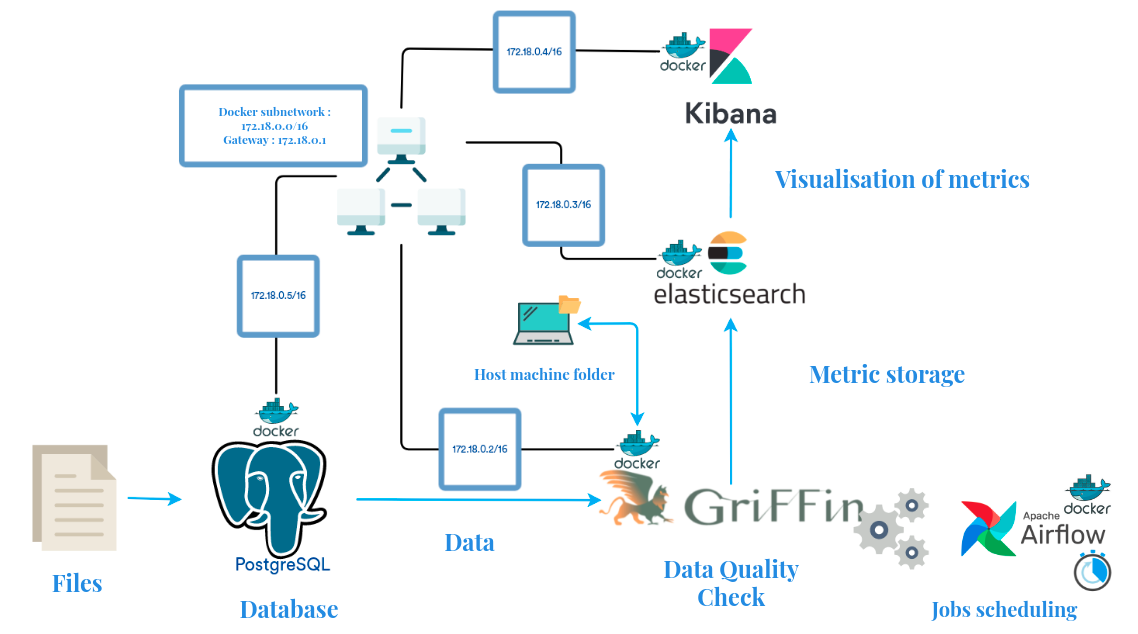
\includegraphics[scale=0.40]{Main/Static/Arch_eng.png} 
    \end{center}
\end{figure}
The installation is done via docker and takes place in two main steps, according to the documentation \cite{ApacheGriffinDocDocker}. First, a preparation of the working environment is required. This step is carried out in three (3) essential points:
\begin{enumerate}[parsep=0cm,itemsep=0cm]
    \item the installation of docker and docker compose;
    \item increasing the virtual memory limits for the use of Elasticsearch;
    \item retrieving the docker images needed for the installation. 
\end{enumerate}
After preparing the environment, the next step is the creation of the different docker containers.

\subsubsection{Connection to PostgreSQL}
Assessing the quality of data obviously requires data. For this purpose, Griffin allows you to configure access to different data sources. In particular, in batch mode, Griffin can audit the quality of data located in Hive tables, AVRO files, flat files (Parquet, \acrfull{csv}, \acrfull{tsv}, \acrfull{orc}) and data from sources with \acrshort{jdbc} (\acrlong{jdbc}) drivers such as Oracle, MySQL, PostgreSQL, etc. However, the connection to a PostgreSQL database was not natively supported.  To remedy this, we have modified the source code of the application. This modification involves adding the PostgreSQL database connection driver to the project dependencies. Then at the level of the test files, it was necessary to adapt the code, so that at the phase of build of the project, the driver once downloaded is suitably added to the Classpath. 

\section{Evaluation of the quality of the Digital Factory's data}
The second phase of the project aims to evaluate the quality of some tables with Griffin and to propose corrective measures where possible. For this purpose, two data extractions were provided. These are the 'Detail\_Victimes' and 'Inventaire\_Sinistre' tables. The 'Detail\_Victimes' table contains the information of all deceased or injured victims of an insurance claim as well as the differents assessments history. The 'Inventaire\_Sinistre' table contains the entire claim inventory, including settlements, reserves, and recoveries. The results of the evaluation are presented along each dimension.

\subsubsection{Uniqueness dimension}
For this dimension, we also highlighted for each targeted column three (3) metrics: the total number of observations in the column, the number of distinct observations and the number of distinct observations appearing more than once. The results of this assessment revealed that there were repetitions in the different columns. However, this did not constitute anomalies. This is due to the fact that the data is derived from the join between several tables.

\subsubsection{Validity dimension}
In this dimension we evaluated three (3) main rules. The objective was to identify the range of variation of the quantitative columns, to define the modalities of the different qualitative columns and to highlight the values presenting problems of encoding of accentuated characters. As a result of the evaluation,  we have highlighted encoding problems in the \textit{'Beneficiaire'} column of the 'Detail\_Victimes' table. The encoding problems as we detected them are characterised by the appearance of '?' in place of accented characters. Thus 'p\`ere' is spelled out as 'p?re' for example.

\subsubsection{Completeness dimension}
We use three (3) metrics to assess this dimension: the total number of rows, the number of incomplete observations and the number of non-zero observations. We have eighty (80) columns with missing values for 'Detail\_Victimes'  i.e. about 86\% of the table's columns, and 39 columns for 'Inventaire\_Sinistre', i.e. about 43\% of the columns.

\begin{figure}[H]
    \caption{Completeness 'Detail\_Victimes'}  \label{fig:xray}
    \begin{center}
      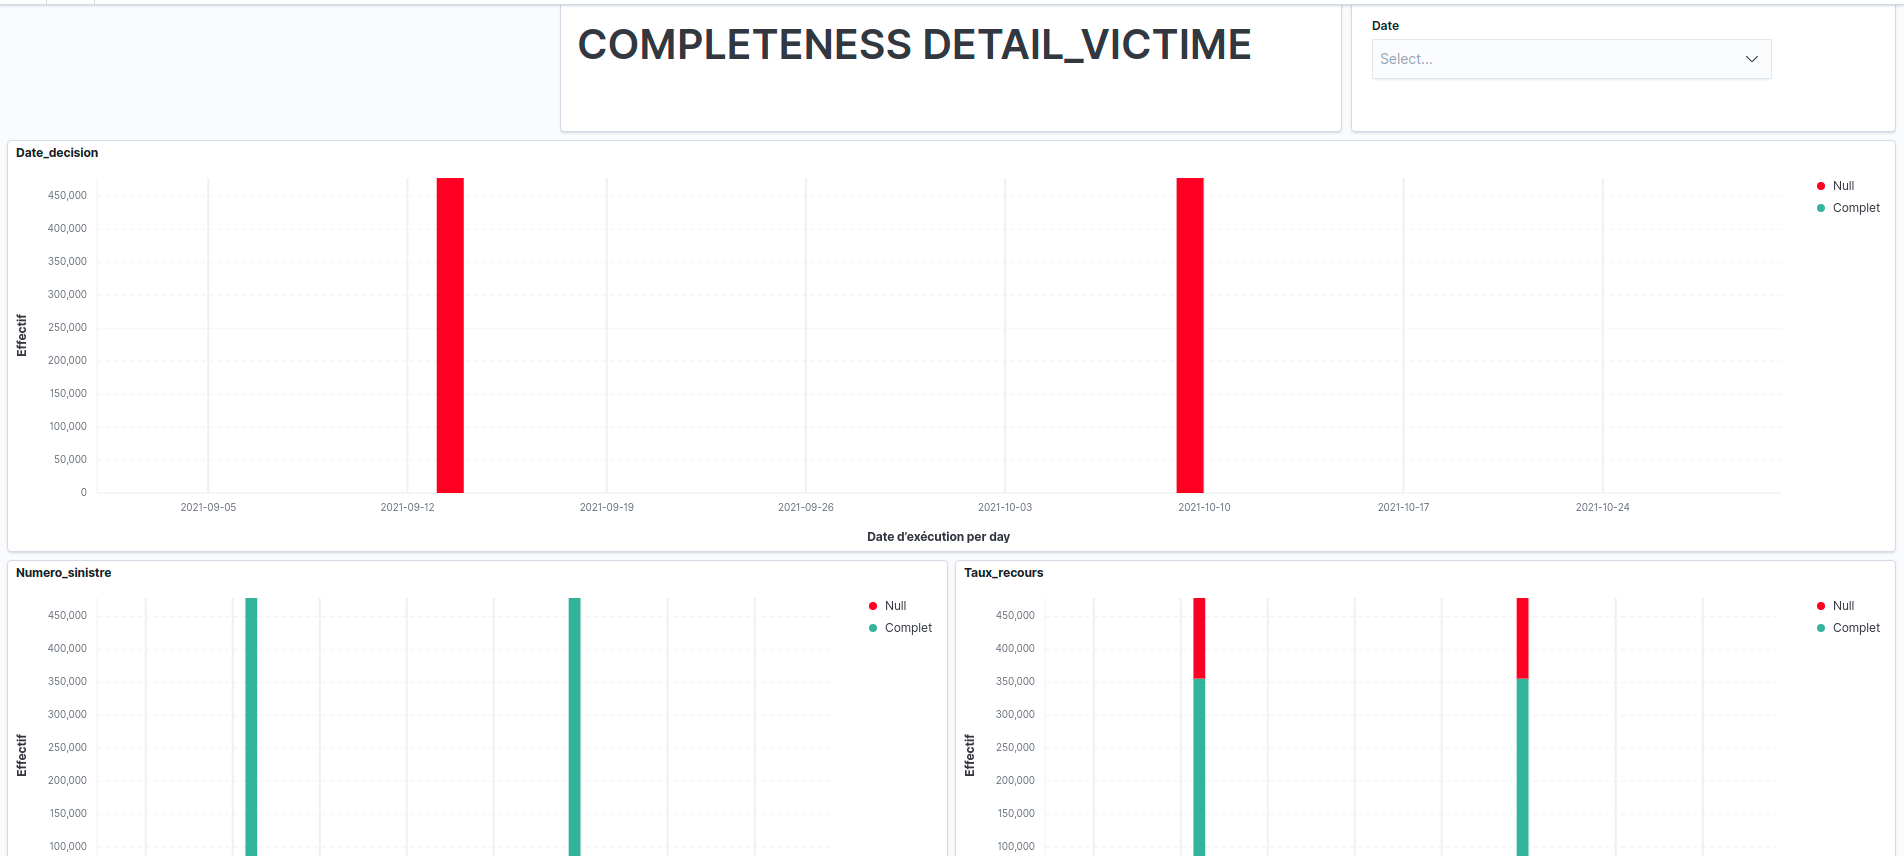
\includegraphics[scale=0.27]{Main/Static/Completeness_Detail_Victime.png} 
    \end{center}
\end{figure}



\subsubsection{Consistency Dimension}
\textbf{'Inventaire\_Sinistre' table}\\
The rules established at the level of this dimension, allow to attest the consistency of the data with the business rules. It is expected that the formulas for the calculation of the charge, the total settlement and the total provision are respected. We also checked the consistency of the dates. Logically, the date of occurrence of the claim, the date of opening of the file and the date of birth of the driver should be earlier than the date of declaration of the claim, the date of closure and the date of licence respectively. In addition to these rules, we have assessed the consistency of the nature of the claim, whether it is 'Bodily' or 'Material'. Indeed, a claim that results in injury and/or loss of life cannot be classified as 'Material'. On the other hand, some claims may be classified as 'Bodily' if they cost more than 100,000 Moroccan dirham even though there are no injuries or deaths. These different rules make it possible to assess the consistency of the nature of the claim. We discovered : 
\begin{itemize}[parsep=0cm,itemsep=0cm] 
    \item 1 claim of a 'Material' nature but with 5 injured victims and 1 deceased;
    \item 237,657 claims with a cost of less than 100,000 Moroccan dirham, with no victims recorded but of a 'Bodily' nature;
    \item 190,622 claims where the number of victims is unequal to the count in the 'Detail\_Victimes' table;
    \item 102 observations for which the claim is declared before it occurs;
    \item 3,972 observations for which the date of obtaining a driving licence is earlier than the date of birth;
    \item 76,000 observations with file opening dates chronologically later than the file closing date.
\end{itemize}
\textbf{'Detail\_Victimes' table}\\
We verify whether the amounts of medical and pharmaceutical expenses and those of permanent partial disability are correctly entered, in accordance with the amount indicator variables. A check has also been made on the consistency of the date of occurrence and declaration. The execution of the rules revealed the following results: 19,082 observations are affected by an inconsistency between the dates of occurrence and declaration. Moreover, when the indicator variable takes the value 'N', meaning that there should be no expenses (medical and pharmaceutical or permanent partial disability), there is sometimes an amount present.

\section{Correction and quality improvement}
The review of the state of data quality identified columns with various anomalies. However, not all of these anomalies constitute errors. Once the selection had been made, we undertook to apply corrections to the columns with consistency problems, as well as a correction of the encoding problems. The various corrections were applied using PySpark (version 2.4.7). This is a Python interface for Apache Spark. 

\subsubsection{Reliability of the number of victims and the nature of the disaster}
In order to correct the differences in the number of injured and deceased victims in the 'Inventaire\_Sinistre' table, the number of injured and deceased victims was counted for each loss in the 'Detail\_Victimes' table. This new data, together with the information contained in the 'Inventaire\_Sinistre' table, produced a new column giving the number of injured and dead for each claim with a corresponding value in the 'Detail\_Victimes' table. With these new values, we proceeded to adjust the nature of the incident. If the number of injured or dead is greater than zero (0), then the claim type is 'Bodily'. Otherwise, if the charge is less than or equal to 100,000 Moroccan dirham and the claim was previously classified as 'Bodily', it is reclassified as 'Material'. Indeed, there is no reason to consider it as a 'Bodily' claim. On the other hand, if none of the above conditions are met and the charge is strictly greater than 100,000 Moroccan dirham or a claim of a 'Material' nature, then the value of the initial variable \textit{'Nature\_Sinistre'} is retained. This adjustment algorithm leads to the creation of a new variable \textit{'Nature\_Sinistre\_New'}.

\subsubsection{Algorithm for correcting encoding problems}
The targets of our correction are the words of the dictionary (not the proper names). The algorithm algorithm used uses Levenshtein's distance to identify the most likely spelling corrections for a word : these are the candidate words. Levenshtein's distance is a measure of similarity between two strings. It is equal to the number of elementary operations to do to transform a string M into a string P. These are :
\begin{itemize}[parsep=0cm,itemsep=0cm]
    \item substitution of a character ;
    \item insertion or addition of a character ;
    \item deleting or erasing a character.
\end{itemize}

Once the list of candidate words has been obtained, the algorithm then compares all the candidates with a dictionary of words. The particularity of this dictionary is that it associates each word with a frequency of occurrence. The key is the word and the value is the frequency of the word. The candidate with the highest frequency of occurrence is more likely to be the correct result. In case of co-occurrence an alphabetical ranking is performed. This algorithm is implemented in Python by the SpellChecker library. 

\subsubsection{Reliability of indicator variables}
Any amount strictly greater than zero (0) must be materialized by the modality 'Y' in the indicator variable. The correction of these inconsistencies is therefore done using the following algorithm: if the amount is greater than zero (0), a new indicator variable is assigned the value 'Y'. Otherwise, the value 'N' is returned to indicate that there is no charge. The correction results in the creation of a new column so that the existing data is not altered. The algorithm implemented allowed the correction of inconsistencies and the imputation of missing values of indicator variables.